% !TeX spellcheck = en_GB
%%=============================================================================
%% Methodologie
%%=============================================================================
\chapter{\IfLanguageName{dutch}{Methodologie}{Methodology}}
\label{ch:methodologie}
In this chapter, the migration from Windows Server 2016 to Windows Server 2019 will be executed. 
This migration will first be performed on an environment which has been based on the Modern Desktop Deployment and Management Lab Kit provided by Microsoft. \autocite{Gallagher2018} 
Here a \acrfull{dc} will be migrated. 
After this, the migration of a typical SAP environment, as described by delaware, from Windows Server 2016 to Windows Server 2019 will be performed. 
Finally, the different versions of the Windows Server 2019 base container images will be analysed. 
How these can lower virtual machine overhead and improve virtualization efficiency compared to their predecessor, will be reviewed. 
But first, the infrastructure that was used for the initial migration will be discussed.

\section{Migrating the \acrshort{os}}
\label{sec:Migrating_the_OS}
In this section, a \acrshort{dc} will be migrated using both the in-place upgrade and side-by-side migration method. 
This to show the basics of the migration process in an environment where no third-party services, such as SAP, are running. 
That will be discussed in Section \ref{sec:SAP}.

\subsection{Technical specifications of the proof of concept environment}
The proof of concept was made using a bare-metal server running Windows Server 2016. 
The proof of concept environment was than virtualized using Hyper-V. 
Additionally, \acrlong{wac} was also installed locally, this to make the management of the resources easier and more efficient.
The specifications of the server are the following:

\begin{itemize}
	\item CPU: Intel Xeon E5620
	\item RAM: 96 GB 
	\item HDD: 500 GB
	\item OS Version: Windows Server 2016
	\item Hyper-V role installed
	\item Administrative rights on the device
\end{itemize}

The proof of concept environment was based on the Modern Desktop Deployment and Management Lab Kit provided by Microsoft. \autocite{Gallagher2018}
This to make replication of the environment simple and efficient.
\\
The Modern Desktop Deployment and Management Lab Kit consists of the components in Table \ref{tab:LKC}.
\\

\begin{table}[ht]
	\centering
	\begin{adjustbox}{width=1\textwidth}
		\begin{tabular}{l|l}
			Server Name  & Roles \& Products                                                  	 \\ 
			\hline
			HYD-DC1      & Active Directory Domain Controller, DNS, DHCP, Certificate Services 	   \\
			HYD-MDT1     & Microsoft Deployment Toolkit                                        		\\
			& Windows 10 1809 ADK                                                 					 \\
			& Windows Deployment Services                                         					  \\
			HYD-CM1      & System Center Configuration Manager 1806                            		   \\
			& Windows Deployment Services                                         						\\
			& Microsoft Deployment Toolkit                                         						 \\
			& Windows 10 1809 ADK                                                 			 			  \\
			& Windows Software Update Services                                        		  			   \\
			& Microsoft SQL Server 2014                                           						    \\
			HYD-APP1     & Microsoft BitLocker Administration and Monitoring                   				 \\
			& Microsoft SQL Server 2014                                          							  \\
			HYD-GW1      & Remote Access for Internet Connectivity                           				   \\
			HYD-INET1    & Simulated Internet                                                			 	    \\
			HYD-VPN1     & Remote Access for VPN                                             				     \\
			HYD-CLIENT1  & Windows 10 1809 Domain Joined                                  					      \\
			& Office 365 ProPlus Build 16.0.11121.20000                         								   \\
			HYD-CLIENT2  & Windows 10 1809 Domain Joined                                     					    \\
			& Office 365 ProPlus Build 16.0.11121.20000                           									 \\
			HYD-CLIENT3  & Windows 10 1809 Workgroup                                         						  \\
			HYD-CLIENT4  & Windows 10 1809 Workgroup                                          						   \\
			HYD-CLIENT5 & Bare metal (no installations)                                      						    \\
			HYD-CLIENT6 & Bare metal (no installations)                                       							 \\
			HYD-CLIENT7  & Windows 7 Domain Joined                                            
		\end{tabular}
	\end{adjustbox}
	\caption[Lab Kit Components]{Modern Desktop Deployment and Management Lab Kit Components}
	\scriptsize	
	Adapted from \cite{MicrosoftCorporation2019}
	\label{tab:LKC}
\end{table}


Only HYD-CLIENT1 will be kept in the environment since there is no need for any additional clients. 
Connection to the \acrshort{vm}s can be made using the credentials in Table \ref{tab:LKCred}.

\begin{table}[ht]
	\centering
	\begin{adjustbox}{width=1\textwidth}
		\begin{tabular}{l|lll}
			User                 & Access Type              & User Name                    & Password \\
			\hline
			Local Administrator  & Administrative           & Administrator                & P@ssw0rd \\
			Domain Administrator & Enterprise Administrator & CORP\textbackslash{}LabAdmin & P@ssw0rd
		\end{tabular}
	\end{adjustbox}
	\caption[Lab Kit Credentials]{Modern Desktop Deployment and Management Lab Kit Credentials}
	\scriptsize	
	Adapted from \cite{MicrosoftCorporation2019}
	\label{tab:LKCred}
\end{table}

\subsection{In-place upgrade to Windows Server 2019}
In this subsection, an in-place upgrade will be performed on the \acrfull{dc}, HYD-DC1, from Windows Server 2016 to Windows Server 2019. 
At first, the operation and services running on the \acrshort{dc}, as well as the connection to the other servers and clients in the domain, will be verified.
\subsubsection{Prerequisites}
Before starting the upgrade, it is important to verify that the server is backed-up. 
Be sure to check when the last back-up was performed and if it can be restored. 
After this, it is important to verify that all the third-party applications on the server are supported by the newest version of the \acrshort{os}, this will be examined for SAP in Section \ref{sec:SAP}. 
Finally, the forest and domain need to be prepared for the upgrade. 
The Windows Server 2019 installation media provides the necessary tools for this. 
The following commands complete this process, as is shown in Figure \ref{fig:Prerequisites}. 
Be sure to verify the mounting point of the installation media, in this scenario it has been mounted to D:\textbackslash{}, change this accordingly on the first line of the commands.

\begin{lstlisting}[breaklines]
:d
cd support\adprep
adprep /forestprep
adprep /domainprep
\end{lstlisting}

\begin{figure}[h]
	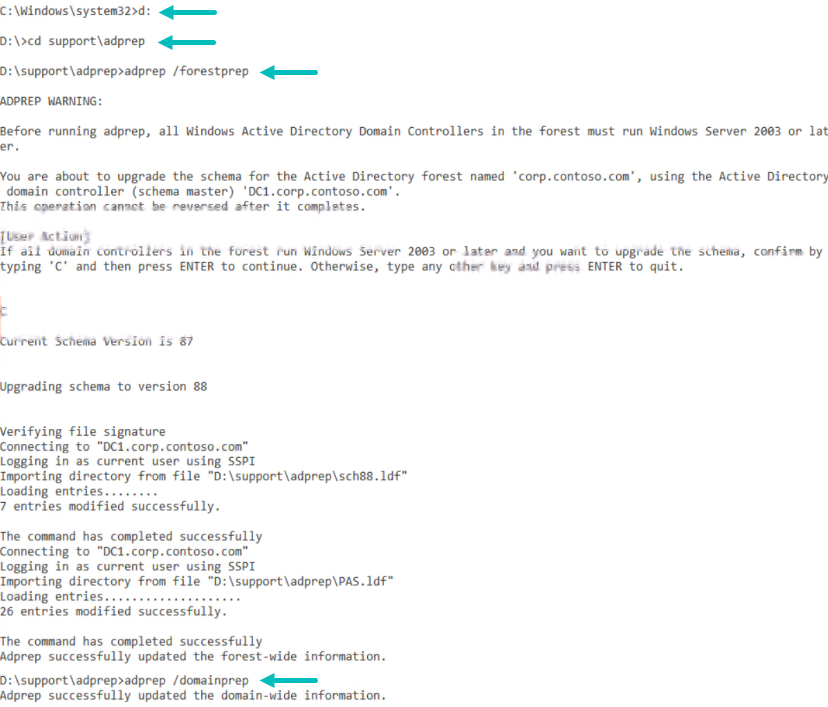
\includegraphics[width=\linewidth]{img/Methodologie/Prerequisites0.png}
	\captionsetup{width=0.9\linewidth}
	\centering		
	\caption[Preparing forest and domain ]{Preparing the forest and domain for in-place upgrade}
	\label{fig:Prerequisites}
\end{figure}
\clearpage

\subsubsection{In-place upgrade}
\label{sssec:In-place_upgrade}
After preparing the forest and domain for the in-place upgrade, the setup from the installation media is to be launched. 
From this point on, the upgrade process has been visualized in Figure \ref{fig:Inplace}. 
Be sure not to use the evaluation version of Windows Server 2019, since this does not support in-place upgrades.

\begin{figure}[h]
	\begin{subfigure}{0.5\textwidth}
		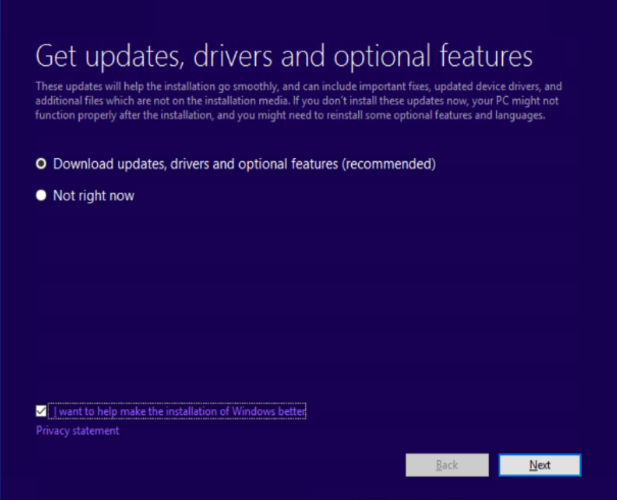
\includegraphics[width=0.9\linewidth,height=4.3cm]{img/Methodologie/InPlace0.png}
		\captionsetup{width=0.8\linewidth}
		\centering		
		\caption{Click next to migrate}
	\end{subfigure}
	\begin{subfigure}{0.5\textwidth}
		\captionsetup{width=0.8\linewidth}
		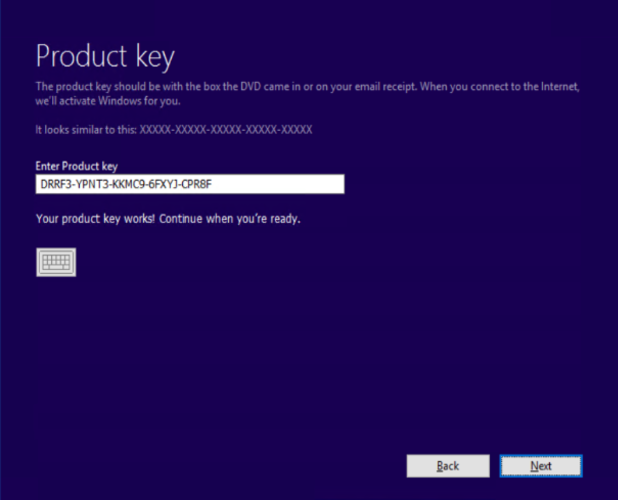
\includegraphics[width=0.9\linewidth,height=4.3cm]{img/Methodologie/InPlace1.png}
		\centering
		\caption{Enter the product key}
	\end{subfigure}
\end{figure}
\begin{figure}[h]\ContinuedFloat
	\begin{subfigure}{0.5\textwidth}
		\captionsetup{width=0.8\linewidth}
		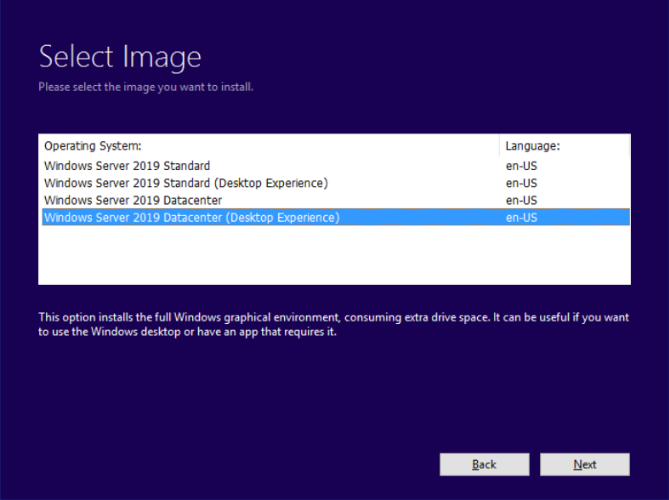
\includegraphics[width=0.9\linewidth,height=4.3cm]{img/Methodologie/InPlace2.png} 
		\centering
		\caption{Select a version of choice}
	\end{subfigure}
	\begin{subfigure}{0.5\textwidth}
		\captionsetup{width=0.8\linewidth}
		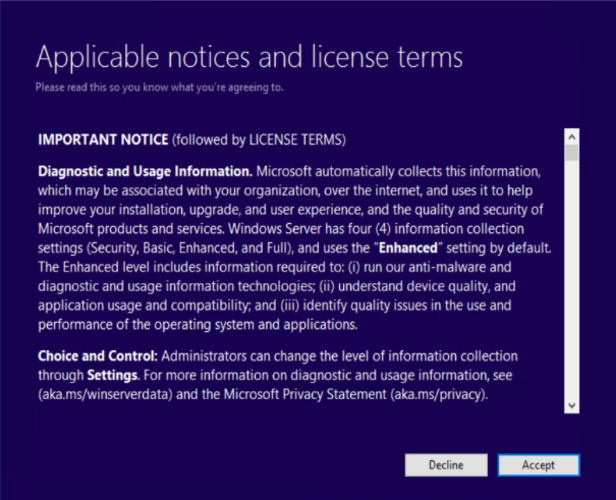
\includegraphics[width=0.9\linewidth,height=4.3cm]{img/Methodologie/InPlace3.png}
		\centering
		\caption{Accept the licence terms}
	\end{subfigure}
\end{figure}
\begin{figure}[h]\ContinuedFloat
	\begin{subfigure}{0.5\textwidth}
		\captionsetup{width=0.8\linewidth}
		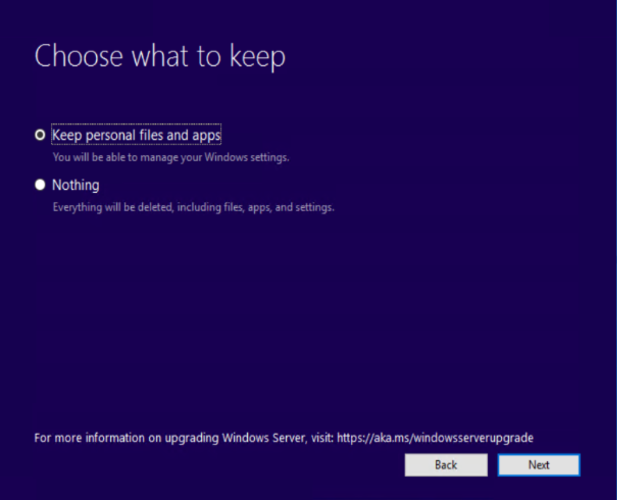
\includegraphics[width=0.9\linewidth,height=4.3cm]{img/Methodologie/InPlace4.png} 
		\centering
		\caption{Select `Keep personal files and apps` to perform an in-place upgrade}
	\end{subfigure}
	\begin{subfigure}{0.5\textwidth}
		\captionsetup{width=0.8\linewidth}
		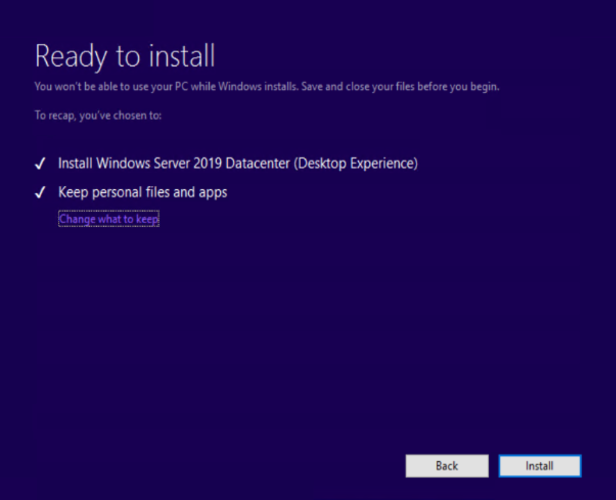
\includegraphics[width=0.9\linewidth,height=4.3cm]{img/Methodologie/InPlace5.png}
		\centering
		\caption{Review the settings and start the installation}
	\end{subfigure}
	\caption[In-place upgrade]{The in-place upgrade process}
	\label{fig:Inplace}
\end{figure}

\subsubsection{Verification}
In this paragraph, the services of the \acrshort{dc}, as well as the connection between the client and server, will be verified. 
First, the \acrfull{rdp} file will be downloaded through the \acrlong{wac}. 
Using this file, a connection to the Hyper-V \acrshort{vm} can easily be made. 
After this, the ability to log in as a domain user is verified, as the \acrshort{dc} provides the login server. 
Afterwards, the domain will be checked through the Control Panel and finally, using Powershell. 
In this final verification, the logon server will be checked as well as how the client is connected to the domain. 
It is expected that the client is connected through the recently upgraded \acrshort{dc}.
The commands, that have been used to verify this, and their expected output can be found below. 
This is also visualized in Figure \ref{fig:Verification}

\begin{lstlisting}[breaklines]
PS C:\Windows\system32> $env:LOGONSERVER
\\DC1
PS C:\Windows\system32> nltest /sc_query:corp.contoso.com
Flags: 30 HAS_IP HAS_TIMESERV
Trusted DC Name \DC1.corp.contoso.com
Trusted DC Connection Status Status = 0 0x0 NERR_Success
The command completed successfully
\end{lstlisting}

\begin{figure}[h]
	\begin{subfigure}{0.5\textwidth}
	\captionsetup{width=0.8\linewidth}
	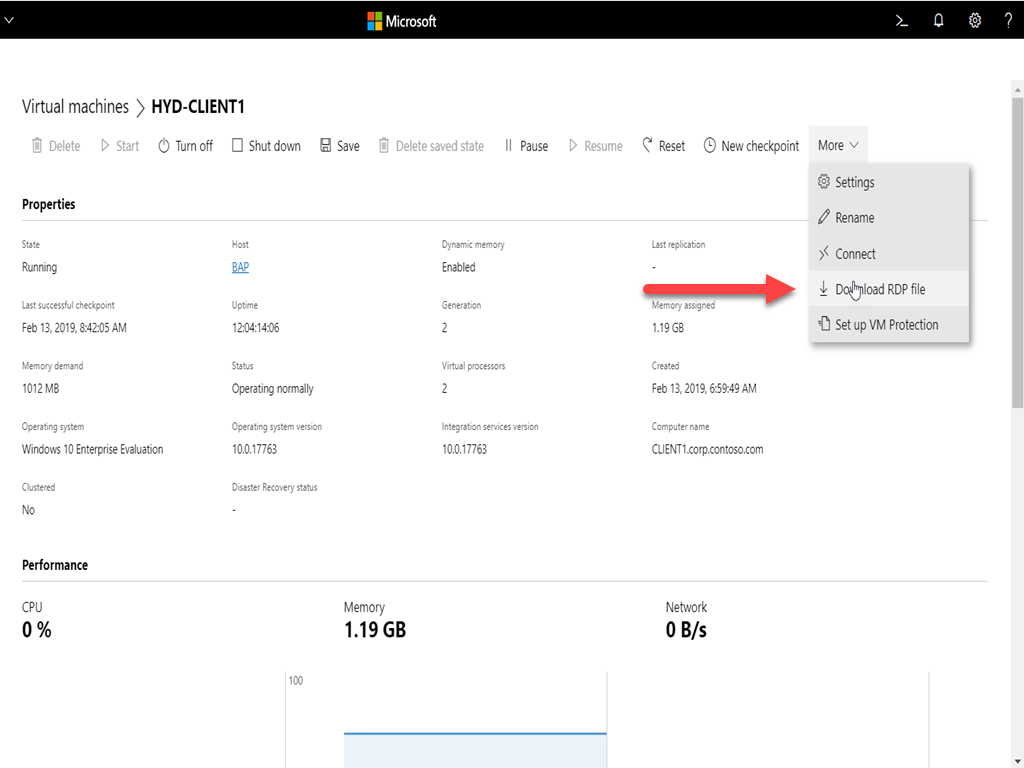
\includegraphics[width=0.9\linewidth]{img/Methodologie/Verification0.png}
	\centering
	\caption{Download and open the \acrshort{rdp} file}
\end{subfigure}
\begin{subfigure}{0.5\textwidth}
	\captionsetup{width=0.8\linewidth}
	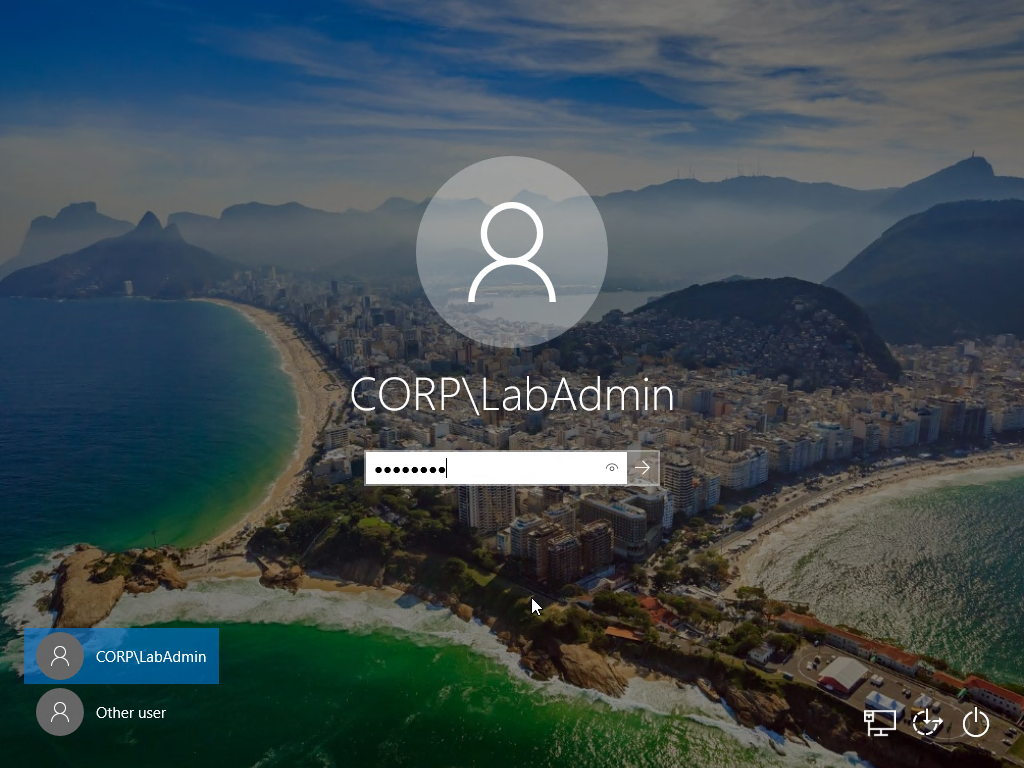
\includegraphics[width=0.9\linewidth]{img/Methodologie/Verification1.png} 
	\centering
	\caption{Log in as a domain user}
\end{subfigure}
\end{figure}
\begin{figure}[h]\ContinuedFloat
	\begin{subfigure}{0.5\textwidth}
		\captionsetup{width=0.8\linewidth}
		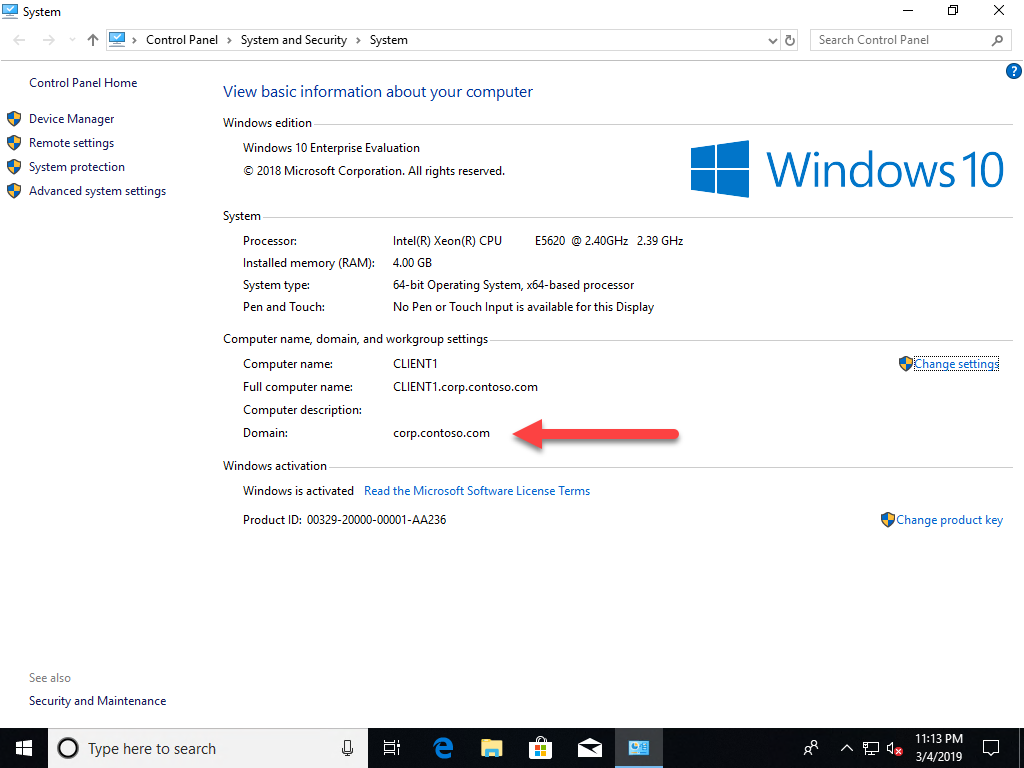
\includegraphics[width=0.9\linewidth]{img/Methodologie/Verification2.png}
		\centering
		\caption{Verify the \acrshort{dc} through the GUI}
	\end{subfigure}
	\begin{subfigure}{0.5\textwidth}
		\captionsetup{width=0.8\linewidth}
		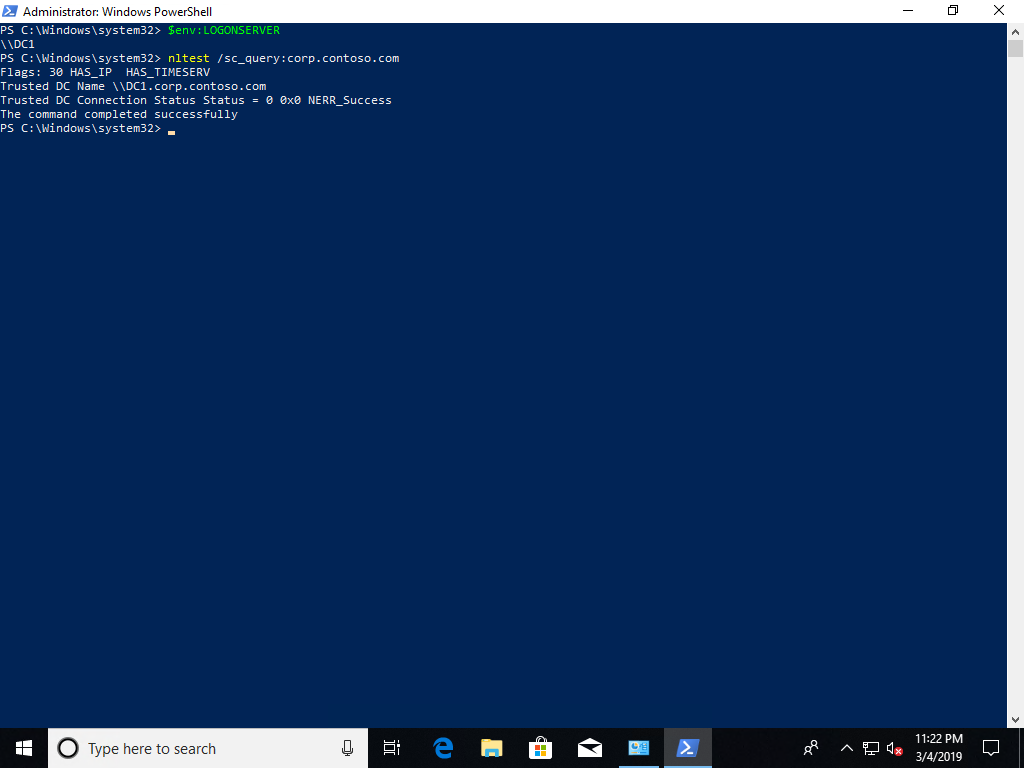
\includegraphics[width=0.9\linewidth]{img/Methodologie/Verification3.png} 
		\centering
		\caption{Verify the \acrshort{dc} through PowerShell}
	\end{subfigure}
	\caption[In-place upgrade verification]{Verifying the connection to the upgraded \acrshort{dc}}
	\label{fig:Verification}
\end{figure}
\clearpage

\subsection{Side-by-side migration to Windows Server 2019}
In this subsection, a side-by-side migration to Windows Server 2019 will be performed on the \acrshort{dc} running Windows Server 2016. 
At first, the connection between the client and the \acrshort{dc} will be verified. 
After this, the side-by-side migration will be performed by creating a new \acrshort{vm} on which Windows Server 2019 will be installed and configured. 
This \acrshort{vm} will, eventually, replace the \acrshort{dc} running Windows Server 2016. 
Finally, the connection between the new  \acrshort{dc} running Windows Server 2019 and the client will be checked.

\subsubsection{Prerequisites}
The connection between the \acrshort{dc} and the client will be verified as was done in Subsection \ref{sssec:In-place_upgrade}.
Additionally, the Windows edition will be checked. 
The prerequisites are shown in Figure \ref{fig:PrerequisitesMigration}.

\begin{figure}[h]
	\begin{subfigure}{0.5\textwidth}
		\captionsetup{width=0.8\linewidth}
		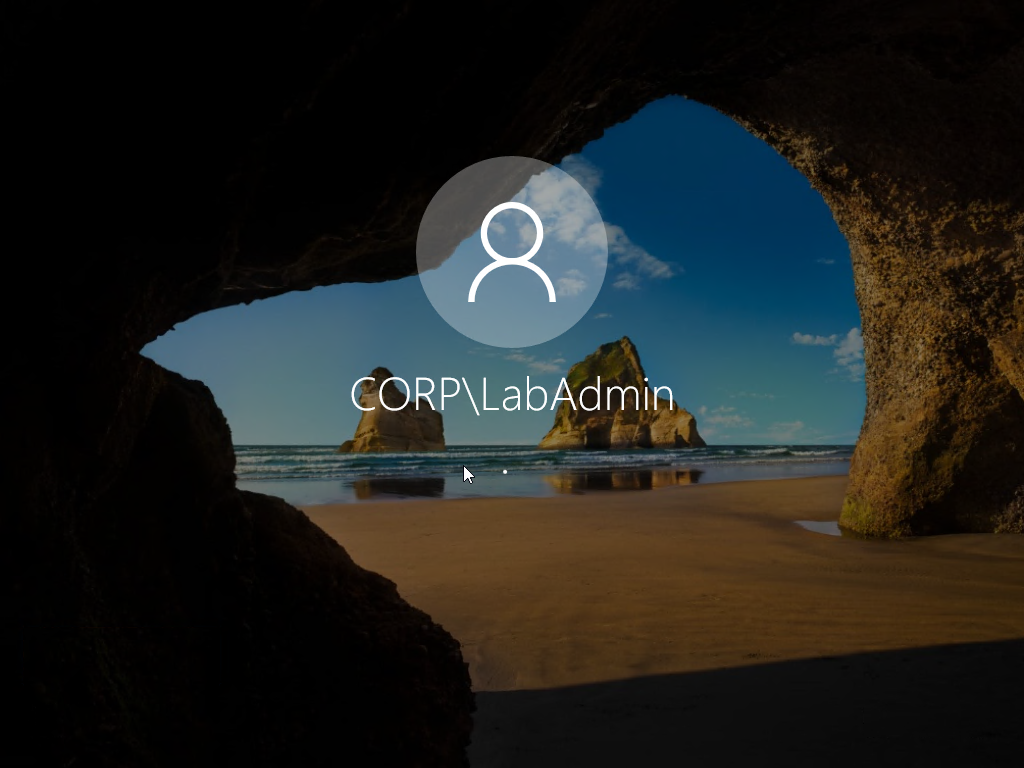
\includegraphics[width=0.9\linewidth]{img/Methodologie/Prerequisites1.png}
		\centering
		\caption{Log in as a domain user}
	\end{subfigure}
	\begin{subfigure}{0.5\textwidth}
		\captionsetup{width=0.8\linewidth}
		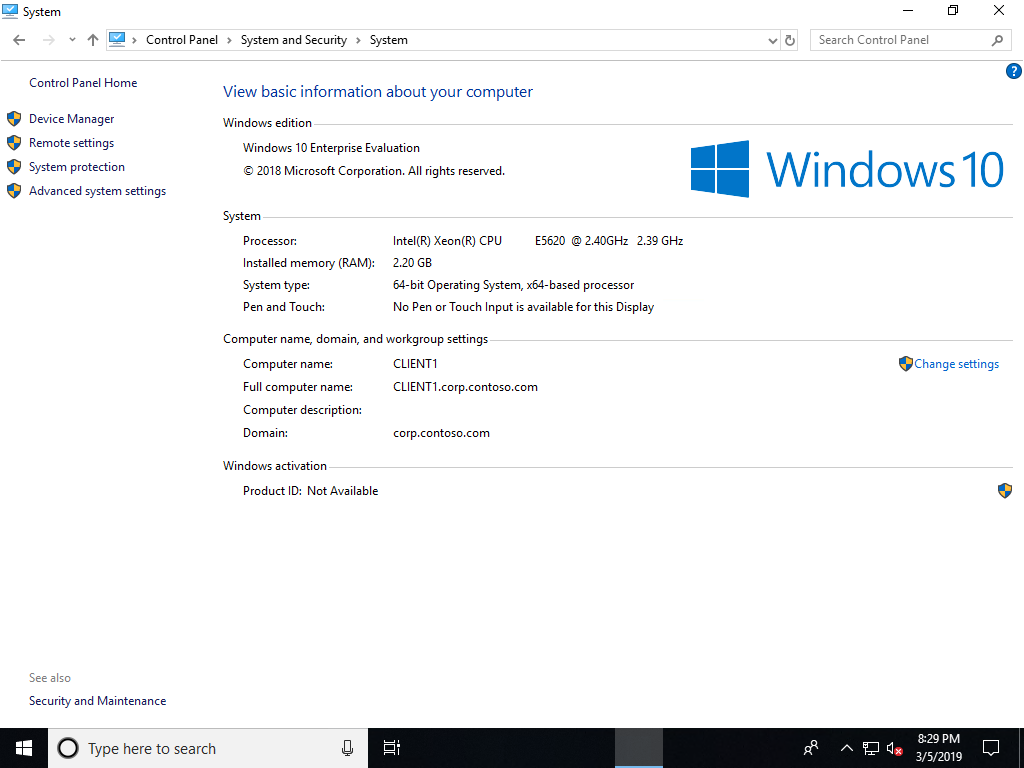
\includegraphics[width=0.9\linewidth]{img/Methodologie/Prerequisites2.png} 
		\centering
		\caption{Verify the \acrshort{dc} through the GUI}
	\end{subfigure}
\end{figure}
\begin{figure}[h]\ContinuedFloat
	\begin{subfigure}{0.5\textwidth}
		\captionsetup{width=0.8\linewidth}
		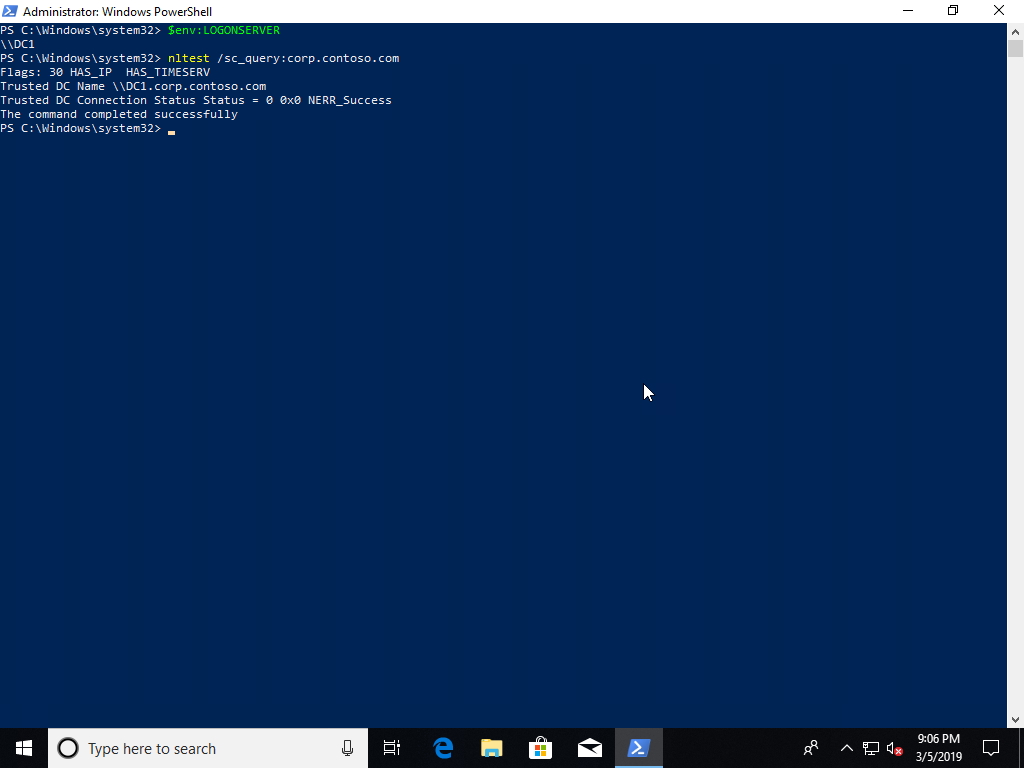
\includegraphics[width=0.9\linewidth]{img/Methodologie/Prerequisites3.png}
		\centering
		\caption{Verify the \acrshort{dc} through PowerShell}
	\end{subfigure}
	\begin{subfigure}{0.5\textwidth}
		\captionsetup{width=0.8\linewidth}
		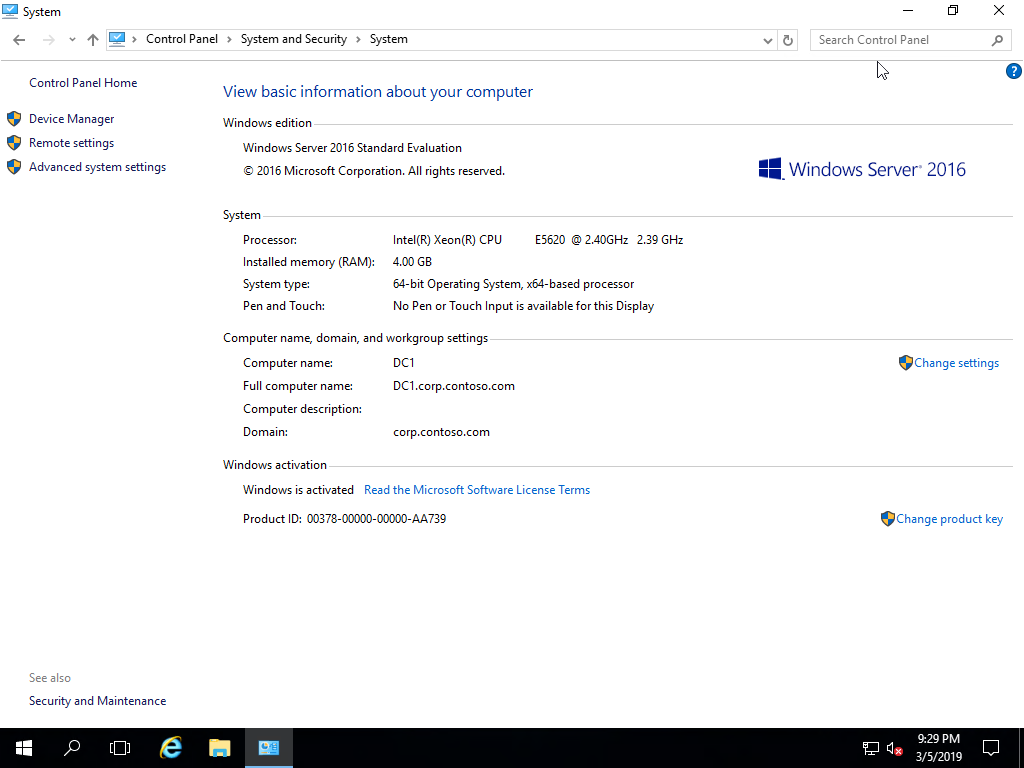
\includegraphics[width=0.9\linewidth]{img/Methodologie/Prerequisites4.png} 
		\centering	
		\caption{Verifying the Windows edition}
	\end{subfigure}
	\caption[Side-by-side migration prerequisites]{Verifying the connection between the client and \acrshort{dc}}
	\label{fig:PrerequisitesMigration}
\end{figure}

\subsubsection{Side-by-side migration}
\label{sssec:Side-by-side_migration}
The side-by-side migration to the new Windows Server 2019 \acrshort{dc}, that will be performed in this paragraph, can be divided into seven parts:
\begin{enumerate}
	\item Creating the \acrshort{vm}
	\item Installing Windows Server 2019
	\item Joining the existing domain
	\item Promoting the new \acrshort{vm} to \acrshort{dc}
	\item Migrating the FSMO roles
	\item Configuring DNS and DHCP
	\item Decommissioning the old \acrshort{dc} 
\end{enumerate}
Considering the magnitude of this side-by-side migration it is not included in the main part of this bachelor's thesis. 
However, it can be found in Appendix \ref{Migration}. 

\subsubsection{Verification}
\begin{figure}[h]
	\begin{subfigure}{0.5\textwidth}
		\captionsetup{width=0.8\linewidth}
		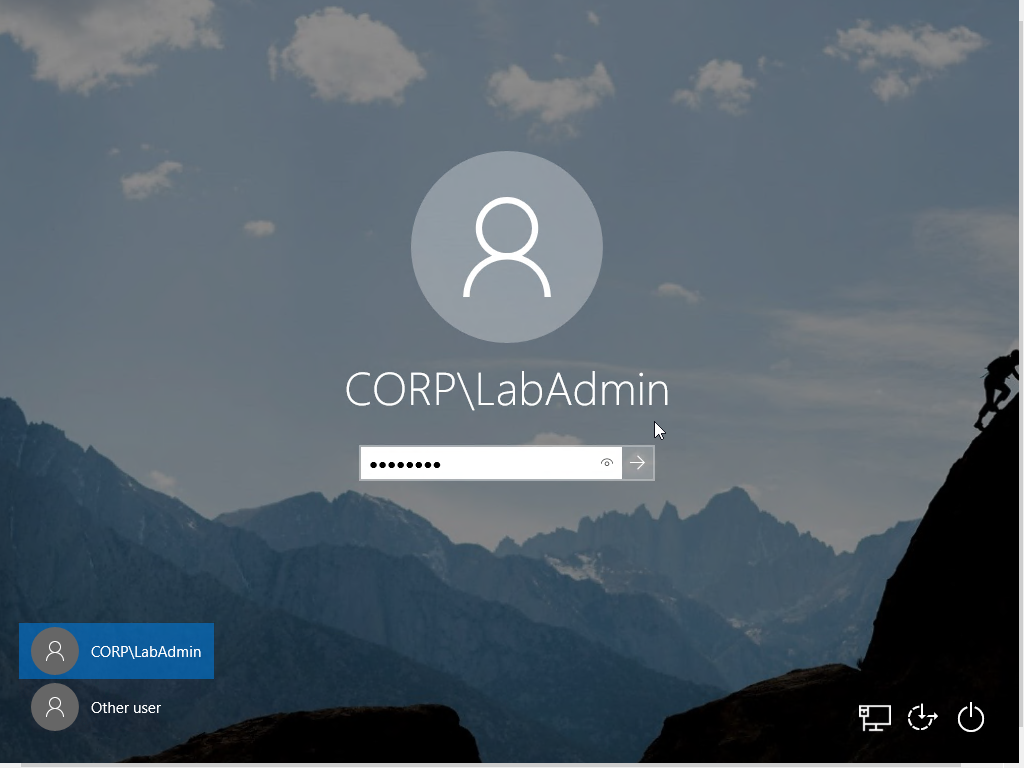
\includegraphics[width=0.9\linewidth]{img/Methodologie/Verification4.png}
		\centering
		\caption{Download and open the \acrshort{rdp} file}
	\end{subfigure}
	\begin{subfigure}{0.5\textwidth}
		\captionsetup{width=0.8\linewidth}
		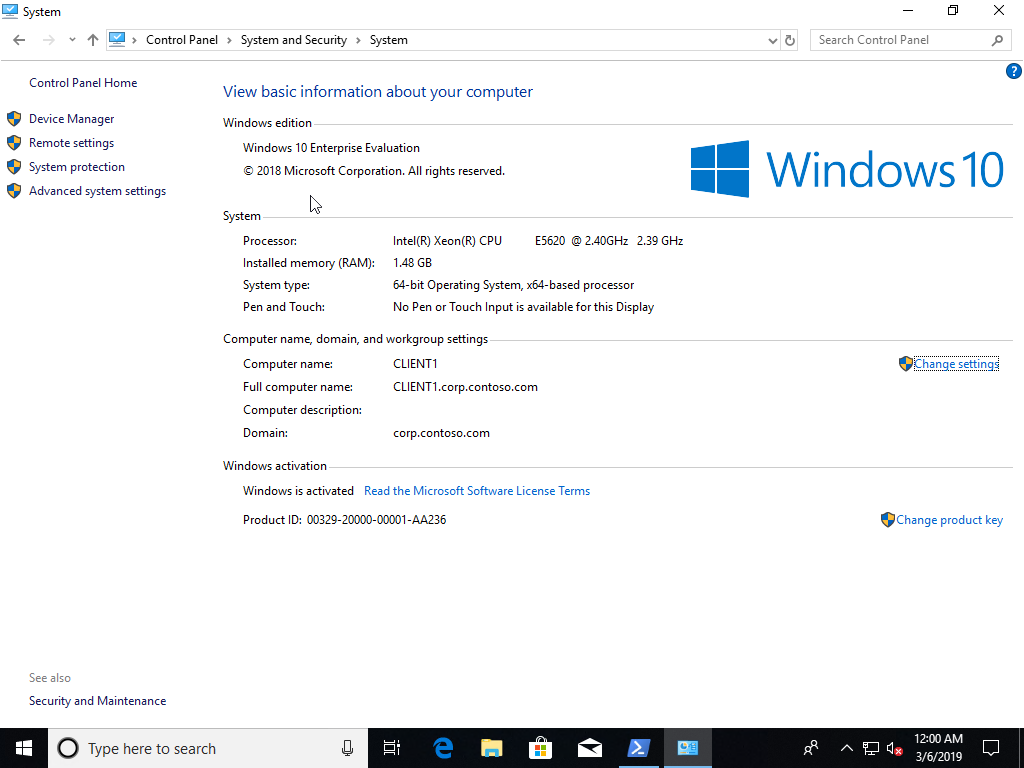
\includegraphics[width=0.9\linewidth]{img/Methodologie/Verification5.png} 
		\centering
		\caption{Log in as a domain user}
	\end{subfigure}
\end{figure}
\begin{figure}[h]\ContinuedFloat
	\begin{subfigure}{0.5\textwidth}
		\captionsetup{width=0.8\linewidth}
		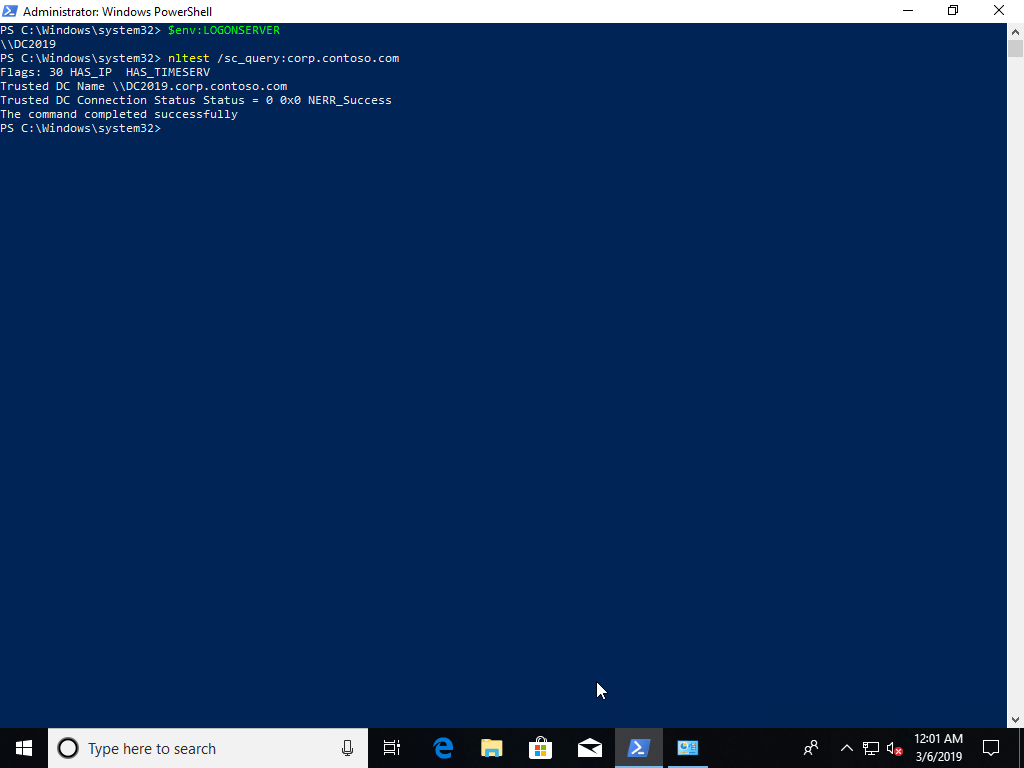
\includegraphics[width=0.9\linewidth]{img/Methodologie/Verification6.png}
		\centering
		\caption{Verify the \acrshort{dc} through the GUI}
	\end{subfigure}
	\begin{subfigure}{0.5\textwidth}
		\captionsetup{width=0.8\linewidth}
		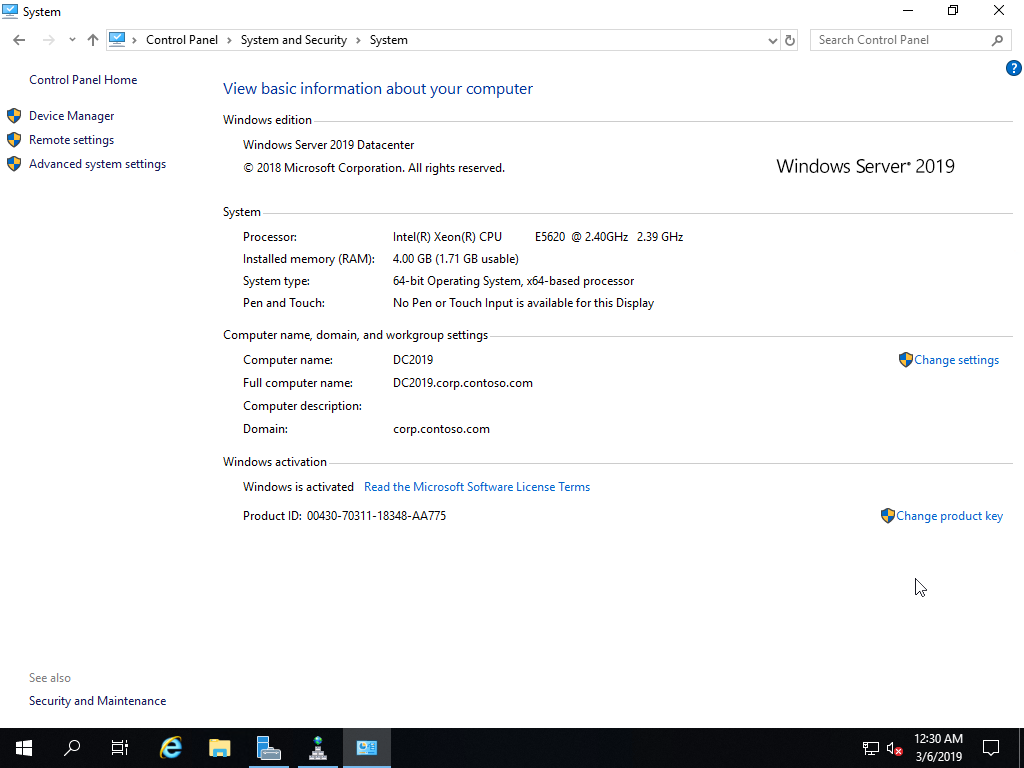
\includegraphics[width=0.9\linewidth]{img/Methodologie/Verification7.png} 
		\centering
		\caption{Verify the \acrshort{dc} through PowerShell}
	\end{subfigure}
	\caption[Verifying the side-by-side migration]{Verifying the connection to the migrated \acrshort{dc}}
	\label{fig:Migration}
\end{figure}
\clearpage

\subsection{Conclusion}
After performing the migration from Windows Server 2016 to Windows Server 2019 using both methods, either of them has its own advantages and disadvantages. 
While an in-place upgrade may seem easier to perform at first glance, it is important to remember that every \acrshort{os} has a certain amount of baggage.
Using this technique these unnecessary files, such as old uninstallers and temporary files, will be transferred from the previous installation to the new one. 
This eventually can have an impact on the performance of the \acrshort{os}. 
It is also important to keep in mind that even though an in-place upgrade might be easier, it cannot be performed from every version to Windows Server 2019.
\\
Using the in-place upgrade from older versions of the \acrshort{os} might require the process to be repeated multiple consecutive times. 
These all increase the additional baggage that gets transferred. 
When choosing for a side-by-side migration this is not the case. 
Only the necessary files and services get transferred to the new \acrshort{os}. 
When choosing for this approach the old infrastructure or \acrshort{vm} can be kept online so that in case of failure everything remains operational. 
Only after extensive testing, the old infrastructure can be taken offline, so that it gets replaced by the newer one. 
This provides an additional fall-back in case of any problems. 
It is important to note that the side-by-side migration currently is the only migration method that is supported for Microsoft Azure \acrshort{vm}s. 
The approach is, however, much broader and requires more research in advance. 
In this part of the proof of concept, only the \acrshort{dc} was migrated. 
This was done effortlessly thanks to the secondary \acrshort{dc}. 
The research that is required to migrate Windows Server to the latest version in a business environment will be done in the following section, for a SAP environment. 
\clearpage

\section{SAP migration}
\label{sec:SAP}
When migrating a server, it is of great importance that the environment around is mapped entirely. 
This to ensure that all dependencies have been met. 
Afterwards, all of those should be verified. 
In this section, the migration from Windows Server 2016 to Windows Server 2019 will be done in a SAP environment. 
This to provide an example of the additional research that comes with the migration of a server that is performing a critical task in a business environment. 
The migration is of interest in any kind of organization for the same reasons that were mentioned before. 
Additionally, SAP recommands the usage of the latest supported version for its software solutions. 
Currently, the latest supported version is Windows Server 2019 \acrshort{ltsc}.

\subsection{Technical specifications of the SAP environment}
The proof of concept environment has been made using Microsoft Azure. 
For the environment a \acrfull{po} system running Netweaver 7.5 on Windows Server 2016 Datacenter Edition using a Sybase database will be used. 
The architecture of the SAP environment can be seen in Figure \ref{fig:SAPInfra}.
The installation and configuration of the SAP environment can be found in Appendix \ref{SAPConfig}.

%TODO Check PAM and revise Figure
\begin{figure}[h]
	\captionsetup{width=0.8\linewidth}
	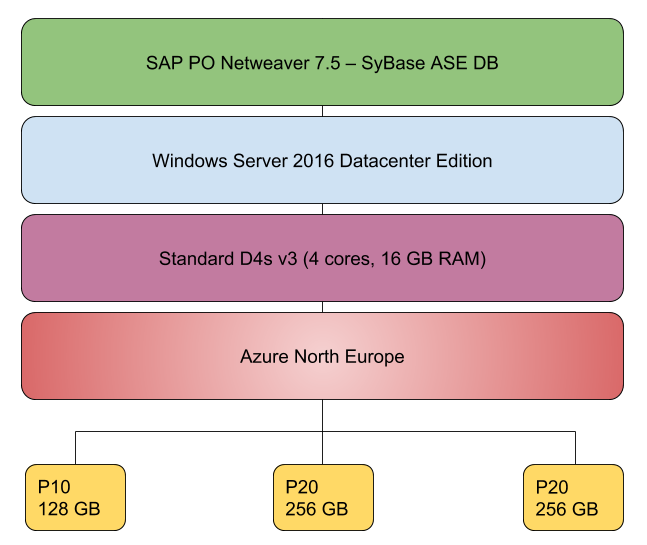
\includegraphics[width=0.9\linewidth]{img/Methodologie/SAP_PO.png}
	\centering
	\caption[SAP Infrastructure]{Infrastructure of the SAP environment}
	\label{fig:SAPInfra}	
\end{figure}

\subsection{Migration of the SAP environment}
%TODO SAP Migration
With Windows Server 2019 SAP offers support for full upgrades. 
This means that for non-clustered systems the in-place upgrade method is supported.
This eliminates the need for a system copy and provides a smooth upgrade to Windows Server 2019. 
However, the traditional method of migration, using the side-by-side migration method, still has the sign of approval. 
Many parts of the migration process that was described in Section \ref{sec:Migrating_the_OS} are applicable to the current environment. 
Because of this reason, the migration of the SAP environment will be kept constraint and the focus will be on the additional chores that come with this migration.

\subsubsection{Prerequisites}
\label{sssec:SAP_Prerequisites}
Before the migration, either it being an in-place upgrade or a side-by-side migration, the operation of the SAP \acrshort{po} solution will be verified.  
The following process will verify the operation of the software solution.

\begin{enumerate}
    \item Browse to `http://host:port/dir`
    \item Click on Enterprise Services Builder
    \item Verify the SAP Basis component as seen in Figure \ref{fig:SAPPreInPlace}
    \item Browse to `http://host:port/pimon`
    \item Click on Adapter Engine
    \item Click on Message Monitor
    \item Verify that no warnings are shown as seen in Figure \ref{fig:SAPPreInPlace}
    \item Browse to `http://host:port/CPACache/refresh`
    \item Execute the cache refresh and verify that no warnings are shown
\end{enumerate}

\begin{figure}[h]
    \begin{subfigure}{0.5\textwidth}
        \captionsetup{width=0.8\linewidth}
        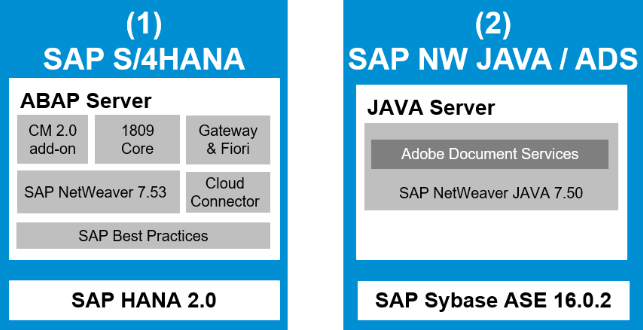
\includegraphics[width=0.9\linewidth]{img/Methodologie/SAP0.png}
        %        TODO SAP1.png
        \centering
        \caption{Verify the SAP Basis component}
    \end{subfigure}
    \begin{subfigure}{0.5\textwidth}
        \captionsetup{width=0.8\linewidth}
        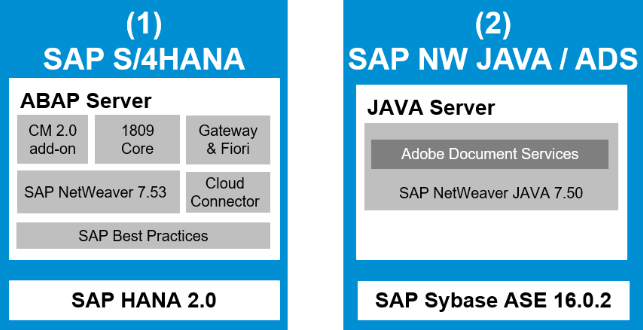
\includegraphics[width=0.9\linewidth]{img/Methodologie/SAP0.png} 
        %        TODO SAP2.png
        \centering
        \caption{Verify that no warnings are shown in Message Monitor}
    \end{subfigure}
    \caption[Prerequisites of the in-place upgrade]{Verifying the operation of the SAP \acrshort{po}}
    \label{fig:SAPPreInPlace}	
\end{figure}

\subsubsection{SAP migration}
After verifying the operation of the software solution, the in-place upgrade will be performed as described in Subsection \ref{sssec:In-place_upgrade}.\\
Alternatively, a side-by-side migration can be performed. 
The side-by-side migration of the SAP environment can be divided into 4 parts:
\begin{enumerate}
    \item Creating the VM
    \item Installing Windows Server 2019
    \item Installing and configuring the SAP environment
    \item Decommissioning the old SAP environment
\end{enumerate}
The first and second part of this procedure were already described in Subsection \ref{sssec:Side-by-side_migration}.
The third part of this procedure has already been described in Appendix \ref{SAPConfig}. 
The final part is the deletion of the old \acrshort{vm} after verifying the operation of the new \acrshort{vm}, as shown in the following paragraph.

\subsubsection{Verification}
After a successful migration, the operation of the SAP \acrshort{po} will be verified, again, as described in Subsection \ref{sssec:SAP_Prerequisites}.

\subsection{Conclusion}
After the migration of the SAP environment, it is clear that many of the aspects from the previous migration in Section \ref{sec:Migrating_the_OS} return. 
With the migration of a software solution it is important to verify that it supports the version of the \acrshort{os} to which will be migrated beforehand. 
For SAP, this was verified using the SAP \acrshort{pam}.
Here all the different aspects that were installed, as described in Appendix \ref{SAPConfig}, were verified to be supported for operation on Windows Server 2019. 
Additionally, verifying the operation of all the third-party applications that need to be installed requires additional research. 
This section of the bachelor's thesis shows that no two migrations are the same. 
It emphasizes that for any migration, irrespective of the size and scope, requires its own research as no environment is identical to the other. 
There are always some variables which should be considered.  
\clearpage

\section{Base container images of Windows Server 2019}
In this final section, a comparison shall be made between the Windows, Server Core and Nano Server base container images. 
At first, the advantages of the new versions of the images will be discussed. 
This involves a comparison between version 1709 and version 1809 of the base container images. 
This will consist of comparing the size and performance of the base container images. 
Afterwards, the different use cases of the various versions will be discussed. 
These base container images have been tested in an environment as described in the following subsection.

\subsection{Technical specifications of the container environment}
The proof of concept environment for the Windows Server base container images was built using the Microsoft Azure platform. 
It uses the Standard D2s v3 (2 vcpus, 8 GB memory) Azure \acrshort{vm}, running the Windows Server 2019 Datacenter Server Core and Containers image.
The following packages will be installed inside the \acrshort{vm}:
\begin{itemize}
	\item Docker
	\item Hyper-V
	\item Windows Containers
	\item Chocolatey
	\item Git
\end{itemize}
The procedure to generate the container environment is described in Appendix \ref{Containers_Azure}.

\subsection{The advantages of version 1809}
With the arrival of version 1809, the \acrfull{sac} equivalent of Windows Server 2019, there have been improvements to the base container images. 
First, the overall size of the base container images has been significantly reduced. 
This can be seen in Figure \ref{fig:Containers}. 
The only exception is the Nano Server image, which has slightly increased in size compared to its previous version. 
This is due to the addition of new features, such as major improvements for Linux containers and container networking through Kubernetes.
The size of the different base images has been obtained by downloading and expanding them as described below. 
This was done through Windows Powershell from inside the \acrshort{vm} that was previously created on the Azure platform. 

\begin{lstlisting}[breaklines]
docker image pull mcr.microsoft.com/windows:1809
docker image pull mcr.microsoft.com/windows/servercore:1809
docker image pull mcr.microsoft.com/windows/nanoserver:1809  
docker image pull mcr.microsoft.com/windows/servercore:1709 
docker image pull mcr.microsoft.com/windows/nanoserver:1709   
docker images | Out-File .container_images.csv
Import-Csv -Path .\container_images.csv
\end{lstlisting}

\begin{figure}[h]
	\captionsetup{width=0.8\linewidth}
	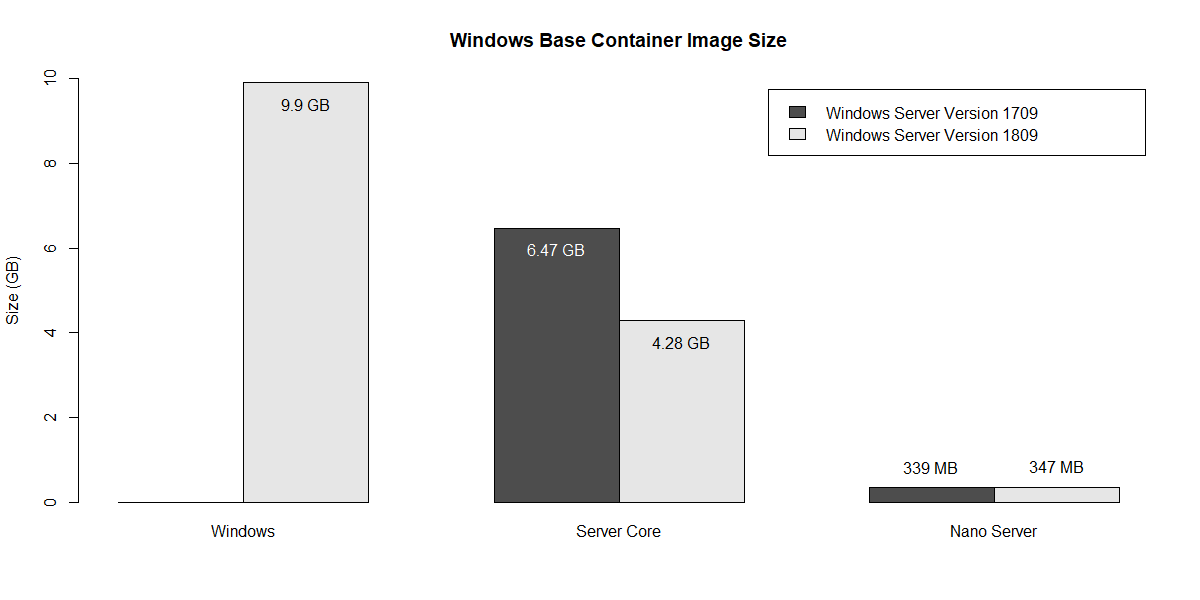
\includegraphics[width=0.9\linewidth]{img/Methodologie/Containers0.png}
	\centering
	\caption[Image size comparison]{Comparison of the Windows base container image size}
	\label{fig:Containers}	
\end{figure}

In this paragraph, the performance of the images shall be tested. 
This will be done using \href{https://benchmarkdotnet.org/}{'BenchmarkDotNet'}, a .NET library made for benchmarking. \autocite{Akinshin2019} 
Benchmarking using this library is done by calculating \acrfull{md5} and \acrfull{sha} hash functions. 
The former is mostly used in the generation of identifiers, as it is not deemed secure enough for data security. 
The latter is better suited for this but has since been improved by \acrfull{sha3}. \autocite{Enkov2017}
\\
The container will be automatically built using a Dockerfile, each of these corresponds with a base container image. 
This is needed to add the required packages inside the container to successfully perform the benchmark. 
For the Windows and Server Core base container image, these were added manually, the Nano Server base container image was provided by Microsoft. 
Following commands need to be executed on the \acrshort{vm} that was created on the Azure platform to benchmark every container individually. 
It is important to note that the kernel version of the \acrshort{os} must match the Windows image. 
While using Hyper-V isolation can circumvent this, it is not recommended since the additional virtualization of the kernel will lower the performance of the container. 
For the unambiguity of the benchmarks, Hyper-V isolation was used.

\begin{lstlisting}[breaklines]
git clone https://github.com/jensdufour/Benchmark.git
cd Benchmark	
docker build -t benchmark1 --isolation=hyperv -f .\WindowsNanoserver1709.dockerfile .
docker build -t benchmark2 --isolation=hyperv -f .\WindowsServercore1709.dockerfile .
docker build -t benchmark3 --isolation=hyperv -f .\WindowsNanoserver1809.dockerfile .
docker build -t benchmark4 --isolation=hyperv -f .\WindowsServercore1809.dockerfile .
docker build -t benchmark5 --isolation=hyperv -f .\Windows1809.dockerfile .
\end{lstlisting}

The results of running the individual benchmarks have been visualized in Figure \ref{fig:MD5} for MD5 and in Figure \ref{fig:SHA} for SHA-256. 
The figures show the average results after running the benchmarks twenty times. 
In Appendix \ref{benchmarkdata}, all the data can be found, as well as the initial results after running the benchmarks ten times. 
Eventual outliers have been removed. 
As can be seen in Figure \ref{fig:MD5} there is no significant difference in performance between the two versions of Nano Server and Server Core.
It is important to note that version 1709 was more performant in this benchmark. 

\begin{figure}[h]
	\captionsetup{width=0.8\linewidth}
	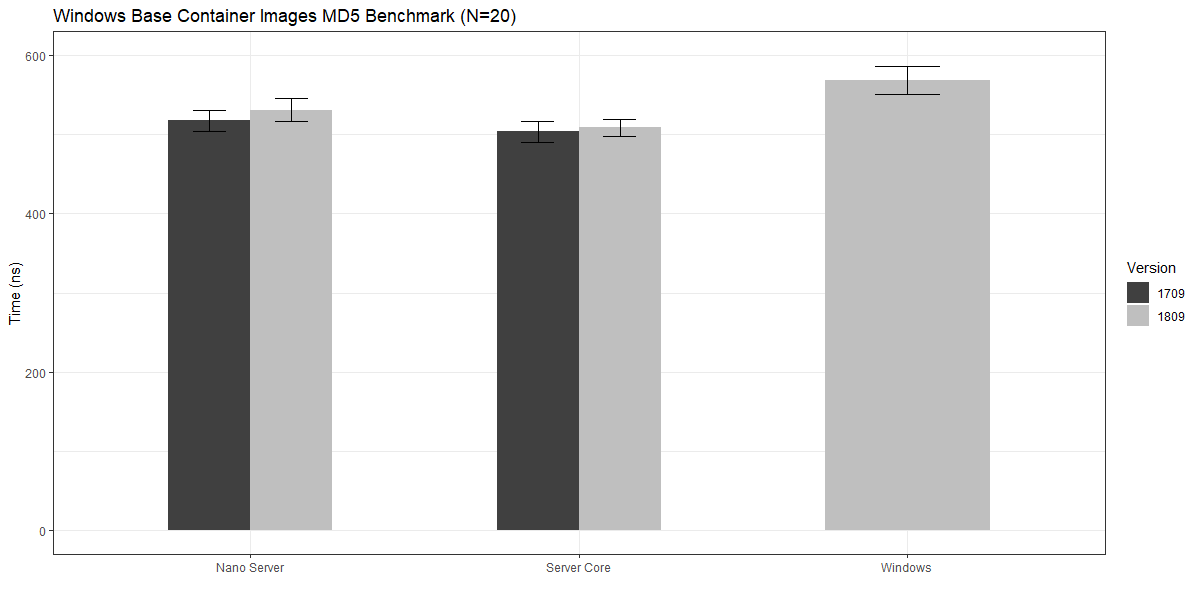
\includegraphics[width=0.9\linewidth]{img/Methodologie/Containers1.png}
	\centering
	\caption[MD5 benchmark]{Windows Base Container Image MD5 benchmark (N=20)}
	\label{fig:MD5}
\end{figure}

In Figure \ref{fig:SHA} similar results can be found. 

\begin{figure}[h]
	\captionsetup{width=0.8\linewidth}
	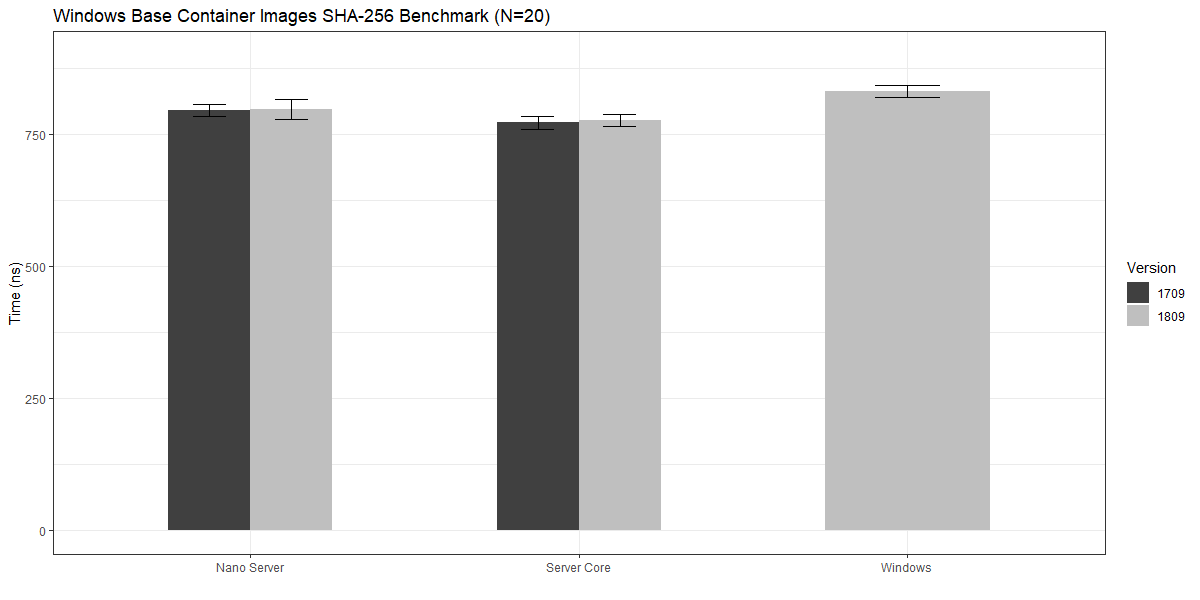
\includegraphics[width=0.9\linewidth]{img/Methodologie/Containers2.png}
	\centering
	\caption[SHA-256 benchmark]{Windows Base Container Image SHA-256 benchmark (N=20)}
	\label{fig:SHA}
\end{figure}

 When looking at the result of the benchmarks of Server Core and Nano Server, the performance of both versions is along the same lines. 
 However, the overall reduction in size and the additional features that have been added, as discussed in Chapter \ref{ch:stand-van-zaken}, make a strong case for the deployment of the latest images, version 1809. 
 The latest release of the base container images also included the Windows base container image. 
 This base container image opens a whole array of new possibilities. 
 The use case of this one and the others will be discussed in the following subsection.

\subsection{Use cases of Windows, Server Core and Nano Server}
The smallest one offered, is the Nano Server. 
This image is aimed at rapid and lightweight deployment using containers. 
It has been specifically designed for `born in the cloud` applications. 
This is a term that has multiple usages, it refers to applications that are not legacy products. 
Applications that provide an agile deployment and offer on-demand availability. 
It is in no way meant to run typical Windows services. 
The bigger brother of Nano Server, Server Core, is more suited for this. 
This image offers application compatibility and has a wide array of built-in Windows roles and features. 
On top of this, it has full .NET Framework support instead of the basic .NET Core that is offered by the Nano Server. 
The final image that is offered is the new kid on the block. 
The Windows base container image offers almost all the Windows components in a lightweight package. 
This makes it exceptionally useful for automated UI tests as it also has DirectX graphics capabilities. 
It also includes a lot of dependencies which make it usable with out-of-date applications which won't be supported in the latest version of Server Core and Nano Server. 
\\
Thanks to the further development to these base container images their footprint has been reduced significantly. 
Although older containers from Windows Server 2016 can still run through Hyper-V isolation on Windows Server 2019, it is recommended to rebuild them with the latest available images.




